\section{Theoretischer Hintergrund des Versuches}
\label{sec:Theorie}

\subsection{Quantenzahlen wasserstoffähnlicher Atome}
\label{subsec:quantenzahlen}
Wasserstoffähnliche Atome (also solche mit einem negativ geladenen und einem
positiv geladenen Teilchen) können durch drei Quantenzahlen charakterisiert
werden. Hierfür verwendet man eine Hauptquantenzahl $n \in \mathbb{N}$, welche das
Hauptenergieniveau des Atoms beschreibt. Die Nebenquantenzahl oder
Bahndrehimpulsquantenzahl $l \in \mathbb{N}_{0} < n$ definiert die Form des
Atomorbitals: $l=0$ für das $s$-Orbital, $l=1$ für das $p$-Orbital etc.
Hierbei gilt: $\sqrt{l(l+1) \hbar}$ ist der Eigenwert des Drehimpulsoperators
$\hat{\vec{L}}$. Die magnetische Quantenzahl $m_{l}$ beschreibt die
z-Komponente des Bahndrehimpulses. Sie kann die Werte
$m_{l} = \frac{L_{z}}{\hbar} = -l,\ldots,-1,0,1,\ldots,l$ annehmen.

\subsection{Feinstruktur und Spin-Bahn Kopplung}
\label{subsec:feinstruktur}
Das den Atomkern umkreisende Elektron kann als Kreisstrom betrachtet werden.
Daher erzeugt es ein elektrisches Dipolmoment. Dieses ist gegeben durch
\ref{eqn:dipolmoment}
\begin{equation}
  \vec{\mu_{L}} = -g_{L} \frac{e}{2m_{e}}\vec{L} = -g_{L}\frac{\mu_{B}}{\hbar} \vec{L}.
  \label{eqn:dipolmoment}
\end{equation}
Hierbei bezeichnet $\mu_{B} = \frac{e \hbar}{2m_{e}}$ das Bohrsche Magneton und $g_{L}$
den Land\'e-Faktor. Dieser hat hier den Wert $g_{L} \approx 1$ und beschreibt das
Verhältnis vom magnetischen Moment und dem Gesamtdrehimpuls.
Für den Betrag des Moments gilt der Zusammenhang
\ref{eqn:dipolmoment_betrag} mit der Nebenquantenzahl $l$.
\begin{equation}
  |\vec{\mu_{L}}| = - g_{L}\mu_{B} \sqrt{l(l+1)}.
  \label{eqn:dipolmoment_betrag}
\end{equation}
Für das gyromagnetische Verhältnis gilt hier \ref{eqn:gyromagnetisch}:
\begin{equation}
  \gamma = \frac{|\mu_{L}|}{|\vec{L}|}.
  \label{eqn:gyromagnetisch}
\end{equation}
Das Elektron besitzt auch einen Spin $S$, welcher ebenfalls ein Dipolmoment
hervorruft. Dieses ist gegeben durch \ref{eqn:dipolmoment_spin}.
\begin{equation}
  \vec{\mu_{S}} = -g_{S} \frac{\mu_{B}}{\hbar} \vec{S}.
  \label{eqn:dipolmoment_spin}
\end{equation}
Hier hat der Land\'e-Faktor den Wert $g_{S} \approx 2$ und gibt das Verhältnis
zwischen magnetischem Moment und dem Spin des Elektrons an.
Für den Betrag des Moments gilt der Zusammenhang
\ref{eqn:dipolmoment_spin_betrag} mit der Spinquantenzahl $s$.
\begin{equation}
  |\vec{\mu_{S}}| = - g_{S}\mu_{B} \sqrt{s(s+1)}.
  \label{eqn:dipolmoment_spin_betrag}
\end{equation}
Für das gyromagnetische Verhältnis gilt hier \ref{eqn:gyromagnetisch_spin}:
\begin{equation}
  \gamma = \frac{|\mu_{S}|}{|\vec{S}|}.
  \label{eqn:gyromagnetisch_spin}
\end{equation}
Die Momente \ref{eqn:dipolmoment} sowie \ref{eqn:dipolmoment_spin}
wechselwirken miteinander. Diese Wechselwirkung wird als Spin-Bahn Kopplung
bezeichnet. Je nachdem, ob die Momente parallel oder antiparallel ausgerichtet
sind, ergeben sich leicht unterschiedliche Energien. Dies trägt zur Aufspaltung
der Energieniveaus in die Feinstruktur bei.

\subsection{Kopplungen in Atomen mit mehreren Elektronen}
\label{subsec:mehrelektronen}
Bei der Betrachtung von Atomen mit mehreren Elektronen ist die Beschreibung
komplexer als für wasserstoffähnliche Atome, da jedes Elektron einen
Bahndrehimpuls $\vec{j}_{i}$ und einen Spin $\vec{s}_{i}$ besitzt. Diese koppeln
auf verschiedene Weisen aneinander. Dies wird im Folgenden für zwei Grenzfälle
beschrieben.

\subsection*{jj-Kopplung}
Bei der jj-Kopplung werden der Bahndrehimpuls $\vec{l}_{i}$ und der Spin $\vec{s}_{i}$ jedes
einzelnen Teilchens zu einem Gesamtdrehimpuls $\vec{j}_{i} = \vec{l}_{i} + \vec{s}_{i}$ addiert.
Aus diesen Gesamtdrehimpulsen der einzelnen Teilchens wird dann der
Gesamtdrehimpuls der Elektronenhülle $\vec{J} = \sum_{i} \vec{j}_{i}$ gebildet.
Die sich ergebenden Zustände sind gute Näherungen für Atome mit starker
Spin-Bahn Wechselwirkung (siehe~\ref{subsec:feinstruktur}).
Die Stärke der Wechselwirkung nimmt mit steigender Ordnungszahl $Z$ zu, sie
ist proportional zu $Z^{4}$. Daher ist die jj-Kopplung für schwere Atome mit
hoher Ordnungszahl eine gute Näherung.
\subsection*{LS-Kopplung}
Bei der LS-Kopplung werden aus den einzelnen Bahndrehimpulsen $\vec{l}_{i}$ und den
einzelnen Spins $\vec{s}_{i}$ die Gesamtbahndrehimpulse
$\vec{L} = \sum_{i} \vec{l}_{i}$ und Gesamtspins $\vec{S} = \sum_{i} \vec{s}_{i}$ gebildet.
Der Gesamtbahndrehimpuls und der Gesamtspin werden dann zu dem Gesamtdrehimpuls
$\vec{J} = \vec{L} + \vec{S}$ kombiniert.
Dies ist eine gute Näherung, wenn die Spin-Bahn Wechselwirkung
(siehe~\ref{subsec:feinstruktur}).
vernachlässigt werden kann. Da die Stärke der Wechselwirkung proportional zu
$Z^{4}$ ist, ist die LS-Kopplung eine gute Näherung für leichte Atome mit
geringer Ordnungszahl. Daher wird in diesem Versuch aufgrund der Verwendung
von Cadmium die LS-Kopplung benutzt.

\subsection{Aufspaltung der Energieniveaus in einem Magnetfeld}
\label{subsec:aufspaltung}
Wenn ein Magnetfeld angelegt wird, kommt es zu der Aufhebung der Entartung in
der magnetischen Quantenzahl $m_{l}$. Dies führt zu einer Aufspaltung der
Energieniveaus und wird als Zeeman-Effekt bezeichnet. Dieser gliedert sich
in zwei Arten, den normalen und den anormalen Zeeman-Effekt.
\subsection*{normaler Zeeman-Effekt}
Der normale Zeeman-Effekt kann beobachtet werden, wenn der Gesamtdrehimpuls
sich nur aus dem Bahndrehimpuls zusammensetzt. Der Spin wird also
vernachlässigt, es gilt $\vec{S} = 0$.
In diesem Fall ist die Wechselwirkungsenergie mit dem äußeren Magnetfeld
gegeben durch~\ref{eqn:energienormal}:
\begin{equation}
  E_{Z,L} = - \vec{\mu}_{L} \cdot \vec{B} = g_{L} \mu_{B} m_{L} B.
  \label{eqn:energienormal}
\end{equation}
Hierbei ist $g_{L} \approx 1$.
Da $m_{L}$ Werte zwischen $-L$ und $L$ annehmen kann (siehe \ref{subsec:quantenzahlen})
ist ein Energieniveau in $2L+1$ äquidistante Energieniveaus aufgespalten.
\subsection*{anormaler Zeeman-Effekt}
Bei zusätzlicher Berücksichtigung des Spins (der Gesamtdrehimpuls setzt sich also
aus Bahndrehimpuls und Spin zusammen) gilt für die
Wechselwirkungsenergie~\ref{eqn:energieanormal}
\begin{equation}
 E_{Z, J} = -\vec{\mu_{J}} \cdot \vec{B} = g_{J} \mu_{B}m_{J} B.
 \label{eqn:energieanormal}
\end{equation}
Für die Berechnung des Land\'e-Faktors gilt~\ref{eqn:lande}
\begin{equation}
  g_{J} = 1 + \frac{J(J+1) + S(S+1) - L(L+1)}{2J(J+1)}.
  \label{eqn:lande}
\end{equation}
Hierbei ist $g_{S} \approx 2$. Der Land\'e-Faktor verändert hier also die Aufspaltung
im Vergleich zum normalen Zeeman-Effekt.

\subsection{Auswahlregeln der Übergänge}
\label{subsec:auswahlregeln}
Zwischen den Zeeman-aufgespaltenen Energieniveaus sind bestimmte Übergänge
möglich. Die Übergänge können durch Auswahlregeln charakterisiert werden.
Diese sind gegeben durch
\begin{align}
  \Delta l &= \pm 1 \\
  \Delta J & =  0, \pm 1 \\
  \Delta m_{J} & = 0, \pm 1.
  \label{eqn:auswahlregeln}
\end{align}
Zusätzlich sind die Übergänge von $J = 0$ zu $J = 0$ sowie von $m_{J} = 0$ zu
$m_{J} = 0$ aufgrund des Pauli-Prinzips verboten. Aufgrund der Beschränkungen
der möglichen Übergänge ergeben sich bei dem normalen Zeeman-Effekt genau drei
Spektrallinien.
Diese Aufspaltungen sind in Abbildung~\ref{fig:uebergang1} für den normalen
Zeeman-Effekt in Cadmium dargestellt.
\begin{figure}[H]
  \centering
  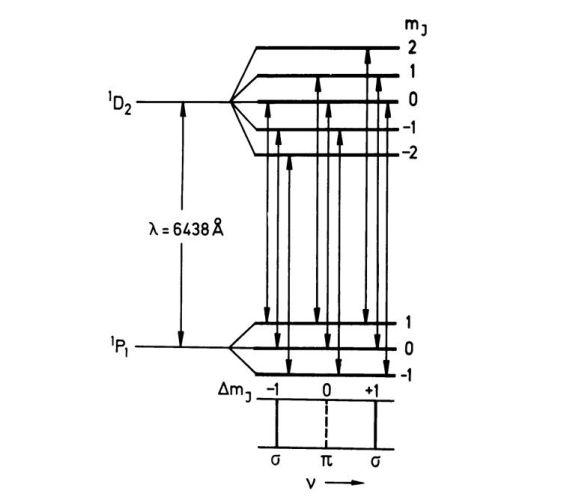
\includegraphics[scale=0.4]{pictures/zeemancadmium1.png}
  \caption{Die Aufspaltung durch den normalen Zeeman-Effekt des Übergangs von $^{2}D_{2} \rightarrow ^{1}P_{1}$ bei $\lambda = \SI{638}{\nano\meter}$. \cite{HakenWolf}}
  \label{fig:uebergang1}
\end{figure}
\noindent
Bei dem anormalen Zeeman-Effekt ergeben sich mehr als drei Energieniveaus.
Wird Cadmium in ein äußeres Magnetfeld gebracht, lassen sich die Aufspaltungen
des Übergangs $^{3}P_{1} \rightarrow ^{3}S_{1}$ beobachten. Diese sind in
Abbildung~\ref{fig:uebergang2} dargestellt.
\begin{figure}[H]
  \centering
  \includegraphics[scale=0.6]{pictures/aufspaltung_blau.png}
  \caption{Die Aufspaltung durch den anormalen Zeeman-Effekt des Übergangs
    von $^{3}P_{1} \rightarrow ^{3}S_{1}$ bei einer Wellenlänge von $\lambda = \SI{480}{\nano\meter}$.}
  \label{fig:uebergang1}
\end{figure}
\noindent
